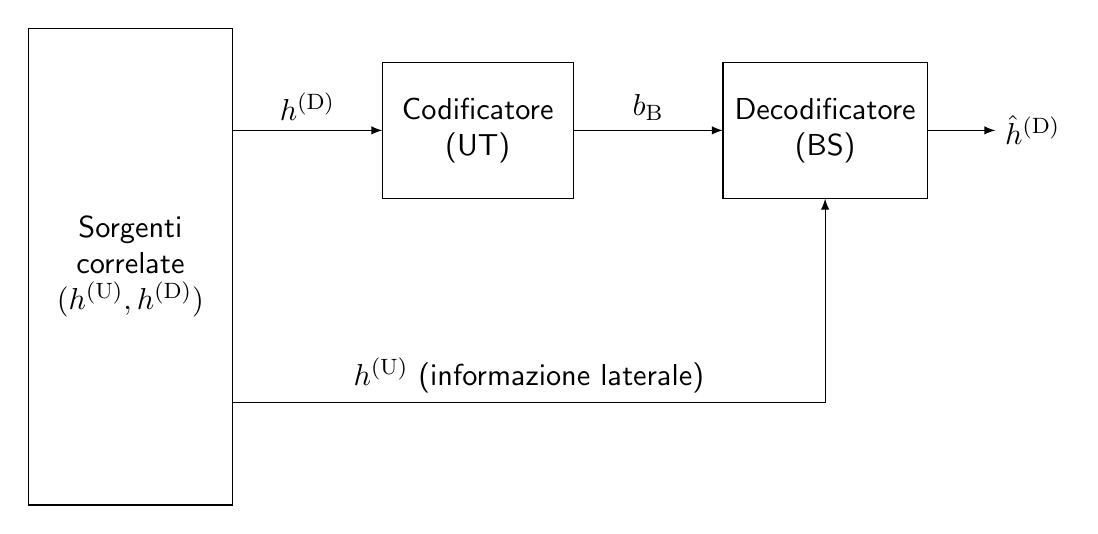
\begin{tikzpicture}[scale=0.865,>=latex]
    \tikzstyle{every node}=[font=\fontsize{11}{13}\sffamily]

    \draw (0,0) rectangle (3,7)
    node[midway,align=center]
    {Sorgenti \\ correlate \\ \((\bm{h}^\mathrm{(U)},\bm{h}^\mathrm{(D)})\)};

    \draw[->] (3,5.5) -- (5.2,5.5)
    node[above,midway]{\(\bm{h}^\mathrm{(D)}\)};

    \draw[-] (3,1.5) -- (11.7,1.5)
    node[above,midway]{\(\bm{h}^\mathrm{(U)}\) (informazione laterale)};

    \draw[->] (11.7,1.5) -- (11.7,4.5);

    \draw (5.2,4.5) rectangle (8,6.5)
    node[midway,align=center]{Codificatore \\ (UT)};

    \draw[->] (8,5.5) -- (10.2,5.5)
    node[above,midway]{\(b_\mathrm{B}\)};

    \draw (10.2,4.5) rectangle (13.2,6.5)
    node[midway,align=center]{Decodificatore \\ (BS)};

    \draw[->] (13.2,5.5) -- (14.2,5.5)
    node[right]{\(\hat{\bm{h}}^\mathrm{(D)}\)};
\end{tikzpicture}
